\documentclass[runningheads]{llncs}
\usepackage[T1]{fontenc}
\usepackage{graphicx}
\usepackage{booktabs}
\usepackage[misc]{ifsym}
\newcommand{\corr}{(\Letter)}
% N.B.: do not change anything above this line. If you require additional packages, please load them directly after this line.
\usepackage{mwe}
\newcommand{\inlineRoot}[1]{\scalebox{0.8}{$\sqrt{#1}$}}
\usepackage{amssymb}
\usepackage{amsmath}
\usepackage{tabularx}
\usepackage{multirow}
% N.B.: you may delete the preceding line. It is used to display an example image in this template.

\begin{document}

\title{Watch Your Step: Realistic Fall Detection in Real-world Streaming Scenarios}

% Really important to test on mobilised data
\titlerunning{Watch Your Step: Realistic Fall Detection in Real-world Streaming Scenarios}
% If the full title of your paper is short enough to also fit in the running head, you can omit the abbreviated paper title here. You can check as follows: if you comment out the \titlerunning line, something will appear in the header of all odd-numbered pages of your PDF from page 3 onward. This something is either the full title (in which case all is well), or the error message "Title Suppressed Due to Excessive Length". If this error message appears, you're going to want to provide an abbreviated title within the \titlerunning command, because if you won't do it, Springer will do it for you.
%N.B.: Author information (both in the \author{} and \authorrunning{} command) should only be present in the Camera-Ready Version of your paper. The version that you initially submit for review, ought to be double-blind. So, when initially submitting your paper, use:
\author{}
% \author{Andr\'e Lauren Benjamin\inst{1} \and
% Calvin Cordozar Broadus Jr.\inst{2,3} \corr \and
% Antwan Andr\'e Patton\inst{1}\orcidID{0000-1111-2222-3333}}
% You may leave out the orcidID information, if you want to.
% Use \corr to indicate the corresponding author. Note the spacing around the \corr command. Only one author can be the corresponding author.
%N.B.: comment out the \authorrunning{} command for the double-blind version of your paper submitted for review. Later, if your paper is accepted, use the command for the Camera-Ready Version.
%\authorrunning{A.L. Benjamin et al.}
% First names are abbreviated in the running head.
% If there is one author, write 'A.L. Benjamin'.
% If there are two authors, write 'A.L. Benjamin and C.C. Broadus Jr.'
% If there are more than two authors, '[...] et al.' is used.
\institute{}
% \institute{Fictional Southern University, Savannah GA 31404, USA \email{\{a.l.benjamin,a.a.patton\}@fsu.fake}
% \and
% Fictional West Coast University, Long Beach CA 90840, USA \email{ccb@fwcu.fake}
% \and
% Secondary European Affiliation, Tiergartenstr. 17, 69121 Heidelberg, Germany
% \email{lncs@springer.com}}
\maketitle         

\begin{abstract}
Real-time fall detection is crucial for enabling timely interventions and mitigating the severe health consequences of falls, especially for older adults.  However, existing methods often rely on simulated data or unrealistic segmentation, hindering their real-world applicability.  Furthermore, efficient computation and robust evaluation metrics tailored to continuous monitoring are essential for practical deployment. This paper introduces a novel real-time fall detection framework that directly addresses these challenges. Leveraging over 24 hours of inertial measurement unit data from 41 participants in the FARSEEING dataset, our approach, based on a efficient state-of-the-art time series techniques, computes fall probabilities in streaming mode without prior knowledge of fall events, eliminating manual feature engineering and preventing future information leakage during training. In addition to evaluation on FARSEEING, we further validate our approach on a continuous 7-day real-world mobility dataset from MobiliseD, containing four falls. Our computationally efficient method achieves an F1-score of 0.89 and a false alarm rate of 0.085 per hour on FARSEEING. This framework offers a significant step towards practical, real-time fall monitoring and improved fall management strategies.

% to add results on MobiliseD

%150--250 words.

\keywords{Fall prediction  \and Time series \and Real-world falls.}
\end{abstract}

\section{Introduction}
Falls constitute a major global health concern, representing the second leading cause of unintentional injury deaths worldwide, claiming an estimated 684,000 lives annually \cite{step_safely_2021}. People living with certain medical conditions and older adults, particularly those over 60, are at the highest risk \cite{vaishya2020falls}. Beyond fatalities, an estimated 37.3 million falls annually require medical attention, placing a significant burden on healthcare systems \cite{camp2024integrating}. Therefore, rapid fall detection is crucial for mitigating the severity of fall-related injuries and facilitating timely interventions. Given this critical need, researchers have explored various approaches to automatically identify fall events.

A fall is an event that results in a person coming to rest unintentionally on the ground, floor, or other lower level \cite{step_safely_2021}. Automatically detecting a fall involves data capture, preprocessing, feature extraction, and classification \cite{liu2023review}. Since falls are unintentional by nature, the first and most important step of fall detection, which is data capture, is challenging. This has resulted in the widespread use of simulated fall data for training fall detection models. However, models trained on simulated falls have been shown to exhibit greatly degraded performance in real-world scenarios \cite{aderinola2024accurate}.

Fall data capture involves recording the daily activities of participants for a set period of time in order to capture the characteristic features of their normal activities of daily living (ADLs) and falls. Such data can be recorded using wearable devices such as inertial measurement units (IMUs), or environmental devices, such as cameras and ambient sensors \cite{gaya2024deep}. However, due to their low-cost, portability, and efficiency, wearable devices are often the capture devices of choice, especially for long-term data capture free-living environments \cite{mohan2024artificial}.

In order to distinguish between falls and ADLs, algorithms use could be threshold-based or machine learning (ML) based. Threshold-based methods such as \cite{de2021wearable} use cut-off values set on the sensor signals commonly have high false alarm rates, which could lead to "false alarm fatigue" \cite{mosquera2020automated}. On the other hand, ML methods such as  use conventional classifiers with manually crafted features \cite{son2022machine}, or deep representation learning \cite{liu2023deep}. Some more recent methods take a hybrid approach of preprocessing signals with set thresholds before passing them to an ML model \cite{fernandez2024edge}. However, most of these methods involve segmentation techniques that require prior knowledge of the occurrence of the fall in the test data, limiting their real-world applicability. Furthermore, developing robust fall detection systems for real-world applications presents unique challenges, including the diversity of fall characteristics and the need for continuous, real-time monitoring.

Despite these advances in fall detection, a major limitation still remains the limited applicability in real-world scenarios, partly due to simulated data and partly due to unrealistic segmentation. Existing methods often struggle to operate effectively in truly real-time, continuous monitoring scenarios. This paper addresses this gap by introducing a novel real-time fall probability framework that operates on continuous sensor data without requiring prior knowledge of fall events. Our main contributions are:

\begin{enumerate}
    \item We present a framework for fall probabilities in streaming scenarios, which can improve fall detection outcomes by reducing false alarms and enabling the potential identification of pre-fall events.
    \item We demonstrate realistic fall detection with fall probabilities on two real-world datasets.
\end{enumerate}

To satisfy conditions ideal for a real-time streaming environment, we perform no segmentation on the test set. Additionally, we perform no feature engineering and use efficient time series techniques. Our approach is evaluated on the FARSEEING dataset \cite{klenk2016farseeing}, a large real-world dataset with 92 fallers (mean age 76.1$\pm$12.6 years) and 208 verified falls captured using inertial sensors (accelerometer data). We also further evaluate models trained on FARSEEING on a continuous 7-day real-world accelerometer dataset of a subject, containing 4 falls. We use a fixed-size overlapping window approach for training. On the test set, we take a streaming approach by sliding over the full signal for each test participant and obtaining the probability of each window being a fall event.

\section{Related Work}
In this section, we discuss recent approaches to fall intervention, namely, reactive approaches, and proactive approaches. While reactive approaches focus on detecting falls as soon as possible after it happens to enable quick response and management, proactive approaches focus on taking measures to prevent falls altogether.
\subsection{Reactive Approaches}
\subsection{Proactive Approaches}
% \subsection{Basket Weaving}
% \subsubsection{Underwater Basket Weaving} Only two levels of
% headings should be numbered. Lower level headings remain unnumbered;
% they are formatted as run-in headings.

% \paragraph{Underwater Basket Weaving Under Difficult Circumstances}
% The contribution should contain no more than four levels of
% headings. Table~\ref{tab1} gives a summary of all heading levels.

\section{Materials and Methods}

\subsection{Datasets}
We evaluate our fall detection techniques using the FARSEEING dataset \cite{klenk2016farseeing}, a large collection of real-world falls. We also evaluated our approach on a dataset containing a continuous 7-day recording of a participant, who fell 4 times during the course of data capture.

\subsubsection{FARSEEING.}

\subsection{Data Preprocessing}
\subsubsection{Aggregation and Standardisation.} First, we aggregated the tri-axial acceleration signals into univariate acceleration magnitudes to alleviate the effects of varying sensor configurations. The acceleration magnitudes are obtained as $M = \inlineRoot{Accel_x^2 + Accel_y^2 + Accel_z^2}$, where $Accel_x$, $Accel_y$, and $Accel_z$ are acceleration values in the anterior-posterior, medial-lateral, and vertical axes respectively. This aggregation reduces the influence of sensor orientation, as the magnitude is invariant to rotations. After aggregation, all signals were standardised to have zero mean and unit variance prior to modeling.

\begin{figure}[t]
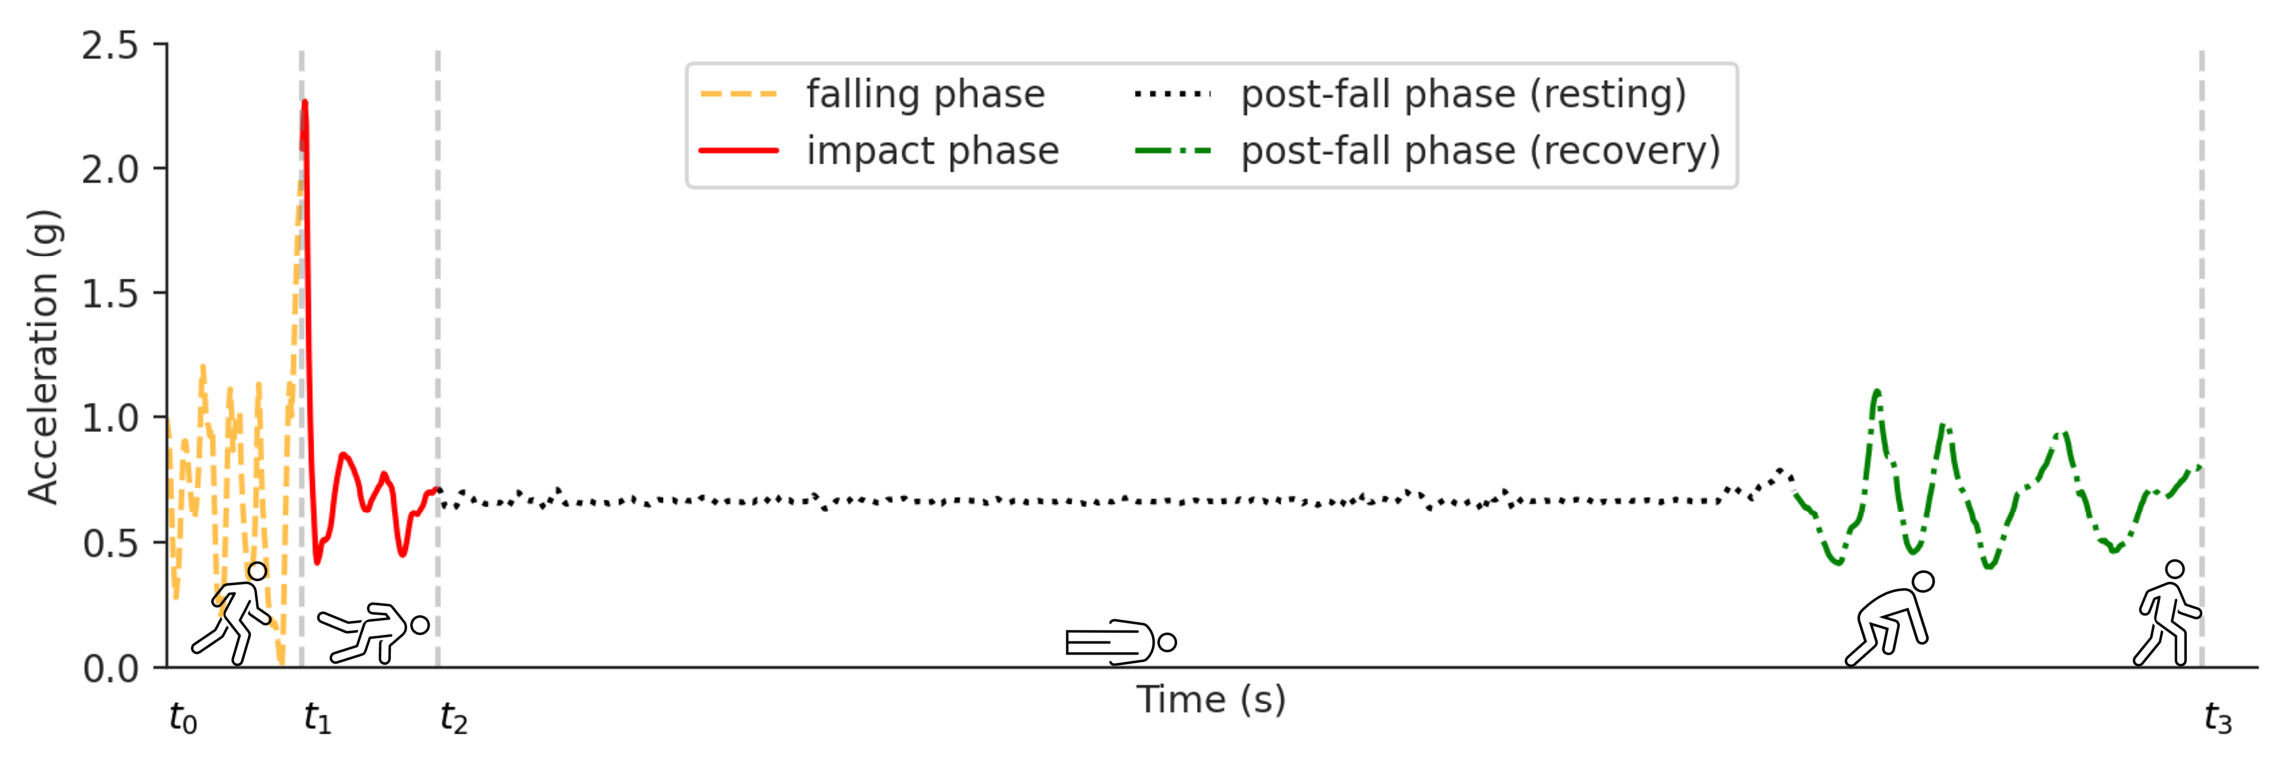
\includegraphics[width=\textwidth]{img/multiphase.pdf}
\caption{A multiphase fall sample from FARSEEING, illustrating the falling, impact, and post-fall phases. The post-fall phase shows the resting period where the faller lies on the ground (the flat region of the signal), followed by the recovery period where the faller begins to get up (indicated by the subsequent increase in signal magnitude).} \label{fig:multiphase}
\end{figure}

\subsubsection{Segmentation for Training.}
The preparation of the training data follows the same procedure as described in our previous work \cite{aderinola2024accurate}. We briefly summarize the key steps here for completeness. A fall is often characterized by a series of events that result in \textit{impact} on the ground, followed by a series of events after impact.  This is well captured in the multiphase fall model proposed in \cite{becker2012proposal}, which we have adopted for fall segmentation. In particular, with a window size of 7 seconds ($t_3 - t_0$), we use a three-phase model: $[t_0, t_1)$, $[t_1, t_2)$, and $[t_2, t_3)$.

\paragraph{Fall Segmentation.} Each fall sample in FARSEEING consists of 20 minutes of accelerometer data centered around the fall event. We extract a segment from $t_0$ (1 second before the impact event) up to $t_3$, where $t_3 = t_0 + window\_size$. As proposed in \cite{palmerini2020accelerometer}, we set the \textit{falling phase} $[t_0, t_1)$ and \textit{impact phase} $[t_1, t_2)$ to 1 second each, such that the duration of \textit{post-fall phase} $[t_2, t_3)$ is 26 seconds. This post-fall phase, illustrated in Fig.~\ref{fig:multiphase}, is crucial for differentiating a fall (impact with the ground) from a near-fall event (e.g., loss of balance without ground impact) as it captures the resting and recovery period.

\paragraph{ADL Segmentation.} Negative samples, representing activities of daily living (ADLs), are extracted from continuous segments of the training data not labeled as falls, using the same 7-second window size. We employ a fixed-sized overlapping sliding window technique with a step size of 1 seconds \textbf{($\approx$ 95\% overlap)}. We select segments where the maximum acceleration magnitude within the $[t_1, t_2)$ window exceeds a threshold $\tau$ of 1.4g. Since acceleration while standing still is around 1g, threshold filters out quiet activities to enhance model robustness.

\subsection{Fall Detection in Streaming Mode}
\label{sec:fall-detection}
To perform fall detection in a streaming setting, we process continuous accelerometer data without any prior knowledge of fall occurrences. We employ a sliding window approach with a 1-second step size and a window size of 7 seconds, consistent with the training data segmentation. For each 7-second window, we compute the probability of a fall event using the trained model.

To obtain fall probabilities, the standardized acceleration magnitude signal within each window is passed to the trained models (described in Section~\ref{sec:experiments}). For windows where the maximum acceleration in $(t_1, t_2]$ is less than 1.4g, the assigned probability is 0. The output of this process is a sequence of probabilities, with each probability corresponding to a 7-second window shifted by 1 second. Since adjacent windows overlap significantly due to the 1-second step size, we apply non-maximum suppression (NMS) to reduce redundancy. Specifically, for each 1-second time point in the signal, we consider all 7-second windows that contain that time point and assign the maximum probability among those windows to that time point. The output of this step is a new sequence of probabilities with the same number of points as the original signal.

\subsubsection{Cost-Sensitive Learning.}
\label{sec:cost-sensitive}
Detecting falls based on computed probabilities requires identifying high-confidence regions where the predicted probability exceeds a predefined threshold  $\tau$. While the default value for  $\tau$ is 0.5, this threshold often needs to be tuned in real-world settings to balance false alarms (FPs) and missed falls (FNs), which have different associated costs. Due to the imbalanced nature of fall detection data and the significantly higher cost associated with missing a fall compared to raising a false alarm, we employ cost-sensitive learning \cite{elkan2001foundations} to optimize  $\tau$.

We define a cost matrix to reflect the relative costs of different outcomes. Let $C_{FP}$ be the cost of a false positive, and $C_{FN}$ be the cost of a false negative.  Based on typical costs, we estimate that false negatives (missed falls) incur costs approximately five times higher than false positives (false alarms), so we set $C_{FN} = 5 C_{FP}$. We use a unit cost ($C_{FP} = 1$), resulting in $C_{FN} = 5$. Normalizing these costs so they sum to 1 (along with a gain of 2 for true positives), our gain matrix $G$ becomes:

\begin{equation}
\label{eqn:gain-matrix}
    G = \begin{bmatrix}
        1 & -1/6 \\  % Normalized cost of FP
        -5/6 & 2    % Normalized cost of FN, gain for TP
    \end{bmatrix}
\end{equation}
where $G_{1,1}$, $G_{1,2}$, $G_{2,1}$, and $G_{2,2}$ are the gains (or costs) associated with true negatives, false positives (FPs), false negatives (FNs) and true positives (TPs) respectively. This cost matrix is constructed so that true positives incur the highest gain, and false negatives are more costly than false positives.

We use this gain matrix to perform cost-sensitive threshold tuning. Using five-fold cross-validation on the training set, we perform a grid search over 100 probability thresholds $\tau \in [0, 1]$ during cross-validation to select the threshold that maximizes the expected gain according to the gain matrix $G$. This tuned threshold is then used to define high-confidence regions in our fall detection algorithm. Within each high-confidence region, we select the first window whose probability is greater than or equal to the maximum probability observed within that specific high-confidence region. This ensures that only distinct fall events are detected, preventing multiple overlapping detections of the same fall event. This post-processing step results in a list $p$ of starting indices of potential fall points.

\begin{figure}[t]
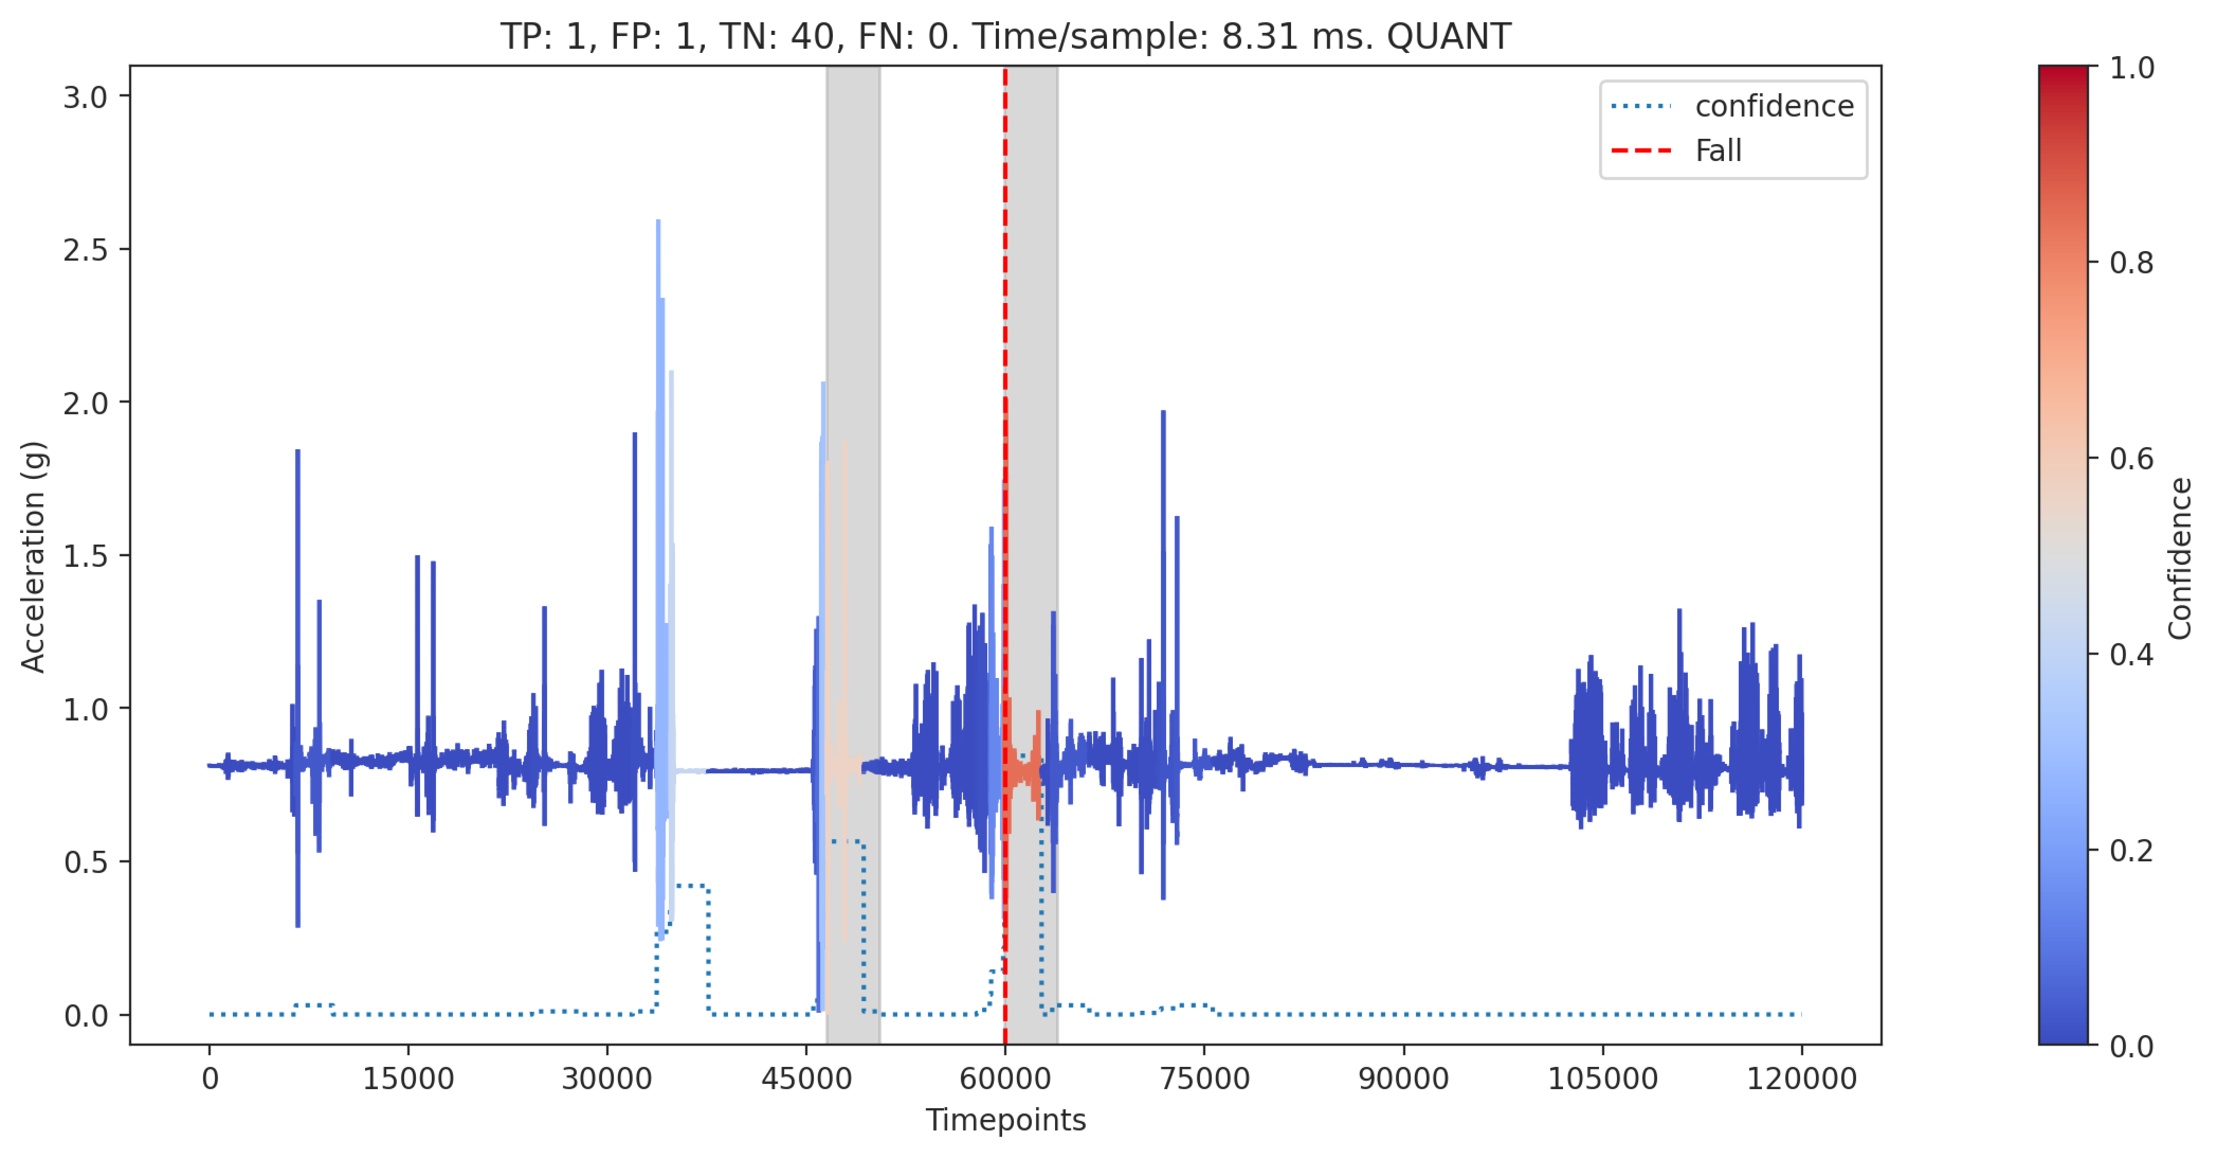
\includegraphics[width=\textwidth]{img/detection_sample.pdf}
\caption{Post-processing of fall probabilities for fall detection, showing each segment of the signal with fall probabilities and predicted falls (shaded windows).} \label{fig:detection_sample}
\end{figure}

\subsubsection{Fall Detection.} Although an impact is marked as a 1-second event (corresponding to the interval $[t_1, t_2)$ in the segmentation), the clinically relevant fall event encompasses a period before and after the impact. We define the ground truth fall event as the $w$-second interval starting 1 second before the impact point: $[f-1, f+(w-1))$. According to \cite{schwickert2017reading}, any fall where the faller is unable to recover within 24.5 seconds of impact could be a fall with more serious complications. While this highlights the importance of the post-impact phase, early detection is crucial for timely intervention. Therefore, we define an asymmetric tolerance window of [-27, +20] seconds around the annotated impact: $R = [f - (w + t), f + t) = [f - 27, f + 20)$, where $f$ is the ground-truth fall point index (corresponding to $t_1$ in the segmentation), $w = 7$ seconds is the window size, and $t=20$ seconds is the tolerance. This asymmetric tolerance window allows detections up to 27 seconds before and 20 seconds after the annotated impact to be considered true positives. This asymmetry prioritises early detection, which is more crucial for timely intervention in real-world fall scenarios, while still allowing for a reasonable delay in detection after the impact. The post-impact tolerance of 20 seconds was chosen to encompass the majority of recovery periods, while also allowing for timely interventions, without leading to overly long tolerance windows. For each potential detection window $d = [p_i, p_i + w)$, where $p_i \in p$, we compute the Intersection over Union (IOU) as:
\begin{equation}
    IOU(d, R) = \frac{{ d \cap R}}{d \cup R}
\end{equation} 
where $d$ represents the detected window and $R$ is the fall range interval. A true positive (TP) is defined as any detection with  $IOU(d, R)>0$ (any overlap). A false positive (FP) is any detection with  $IOU(d, R)=0$ (no overlap). A false negative (FN) occurs if there is no $d$ such that $IOU(d,R) > 0$ for a given fall event (see Fig.~\ref{fig:detection_sample}).

\section{Experiments}
\label{sec:experiments}
% Todos
% 5. Testing on another dataset--mobiliseD

Although we performed all experiments using Python 3.11.9 using a Linux server running Ubuntu 22.04.3 LTS (1.5TB RAM, 24GB NVIDIA GPU GeForce RTX 4090 GPU), we choose models that require no specialized hardware to run, prioritizing efficiency and accessibility for real-time inference in diverse deployment settings. We perform our initial cross-validation experiments (Section \ref{sec:cross-validation})  using tabular classification models implemented in scikit-learn v1.5.0 \cite{pedregosa2011scikit} and time series classifiers implemented in aeon v0.8.1 \cite{middlehurst2024aeon}, training and evaluating on the FARSEEING real-world falls dataset. 

\subsection{Model Training and Evaluation}
\label{sec:training-and-eval}
\paragraph{Training.} We use a window size of $w = 7$ seconds. With FARSEEING's sampling frequency of $f = 100$ Hz, this results in vectors of length $T = 700$. We perform no feature extraction, representing each segmented sample as a vector $\textbf{x} \in \mathbb{R}^T$. Each sample is labeled with a binary target $y_{train}$ indicating the presence or absence of a fall. Therefore, the training set can be described as $\{X_{train} \in \mathbb{R}^{N \times T}, y_{train} \in \{0,1\}^N \}$.

\paragraph{Testing.} The test set consists of $S$ unsegmented signals, each of length $L$. Each test signal has one fall, annotated with a ground truth impact index $f$. For evaluation purposes, we define a tolerance window of $(f-(w+20), f+20] = (f-27, f+20]$ seconds around the impact index. Any detection window overlapping with the tolerance window around the 1-second ground truth fall event is counted as a true positive (see Section~\ref{sec:fall-detection} for more details).

\paragraph{Evaluation.} We use AUC, Precision, Recall, False Alarm Rate (FAR), and Miss Rate (MR) as evaluation metrics. Scores are reported as mean $\pm$ standard deviation in cross-validation experiments. AUC provides an overall measure of discriminative power, while Precision, Recall, and F$_1$ Score capture the trade-off between correctly identifying falls and minimizing false alarms. FAR and MR quantify the rate of false alarms and missed falls per hour, which is crucial for real-world deployment.

\subsection{Results}
\label{sec:results}
\subsubsection{Cross-validation Results.}
\label{sec:cross-validation}
On the FARSEEING dataset, we use five-fold subject-wise cross-validation with 8 subjects per fold. For each fold, we use the unsegmented signals from the subjects in the fold for testing while segmenting and training on the samples obtained from the remaining subjects. We use the scikit-learn implementations of three tabular classifiers, namely, \textit{ExtraTrees} with 150 estimators, \textit{LogisticRegressionCV} ($CV=5$), and \textit{RandomForest} with 150 estimators. We also use the aeon toolkit implementation of three time series classifiers, namely, \textit{Catch22} \cite{lubba2019catch22}, \textit{Rocket} \cite{dempster2020rocket}, and \textit{Quant} \cite{dempster2024quant}. We evaluate each dataset on all the tabular models using a five-fold-subject cross-validation, using a probability threshold of 0.5. We also ensemble each category of classifiers by using the mean probabilities obtained from each model: \textit{Tab Ensemble}, the ensemble of the three tabular classifiers, and \textit{TS Ensemble}, an ensemble of the three time series classifiers. The cross-validation results are summarised in Table~\ref{tab:cross-val-results} and shown as a boxplot in Fig.~\ref{fig:cross-val-boxplot}.

\begin{table}[t]
\centering
\caption{Mean and standard deviation of metrics across 5-fold subject-wise cross-validation on FARSEEING.} \label{tab:cross-val-results}
\begin{tabularx}{0.96\textwidth}{l  @{\extracolsep{\fill}}  c  @{\extracolsep{\fill}}  c  @{\extracolsep{\fill}}  c  @{\extracolsep{\fill}}  c  @{\extracolsep{\fill}}  c}
\toprule
Model & AUC & Precision & Recall & Specificity & F$_1$ Score \\
\midrule
ExtraTrees & 0.85 $\pm$ 0.03 & 0.87 $\pm$ 0.07 & 0.71 $\pm$ 0.06 & 1.0 $\pm$ 0.0 & 0.78 $\pm$ 0.05 \\
LogisticCV & 0.85 $\pm$ 0.06 & \textbf{0.91 $\pm$ 0.08} & 0.69 $\pm$ 0.12 & 1.0 $\pm$ 0.0 & 0.78 $\pm$ 0.08 \\
RandomForest & 0.9 $\pm$ 0.03 & 0.85 $\pm$ 0.09 & 0.81 $\pm$ 0.06 & 1.0 $\pm$ 0.0 & 0.82 $\pm$ 0.02 \\
Tab Ensemble & 0.87 $\pm$ 0.03 & 0.9 $\pm$ 0.03 & 0.75 $\pm$ 0.05 & 1.0 $\pm$ 0.0 & 0.81 $\pm$ 0.03 \\
Catch22 & 0.84 $\pm$ 0.04 & 0.8 $\pm$ 0.16 & 0.68 $\pm$ 0.08 & 1.0 $\pm$ 0.0 & 0.72 $\pm$ 0.07 \\
\textbf{QUANT} & \textbf{0.92 $\pm$ 0.04} & 0.9 $\pm$ 0.04 & \textbf{0.83 $\pm$ 0.07} & 1.0 $\pm$ 0.0 & \textbf{0.86 $\pm$ 0.06} \\
Rocket & 0.9 $\pm$ 0.05 & 0.78 $\pm$ 0.12 & 0.80 $\pm$ 0.10 & 1.0 $\pm$ 0.0 & 0.78 $\pm$ 0.09 \\
TS Ensemble & 0.9 $\pm$ 0.03 & 0.88 $\pm$ 0.06 & 0.80 $\pm$ 0.06 & 1.0 $\pm$ 0.0 & 0.84 $\pm$ 0.04 \\
\bottomrule
\end{tabularx}
Best model (based on F$_1$ Scores) and best metrics are shown in \textbf{bold}.
\end{table}

\begin{figure}[h]
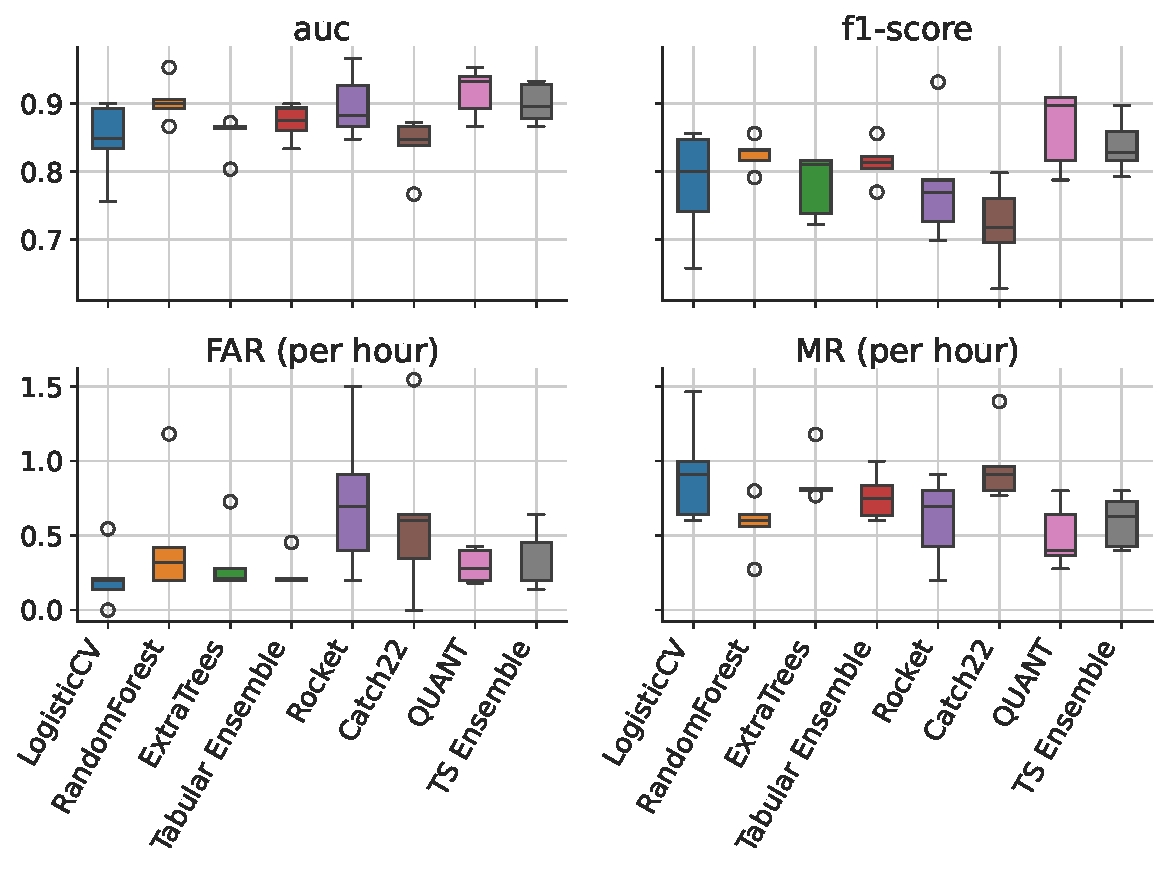
\includegraphics[width=\textwidth]{img/farseeing_metrics_boxplot.pdf}
\caption{Cross-validated AUC, F$_1$ Scores, false alarm rate, and miss rates for all models.} \label{fig:cross-val-boxplot}
\end{figure}

\subsubsection{Cost-sensitive Learning for Threshold Tuning.}
In addition to the standard metrics, we use a gain metric $g$ that reflects the costs defined in our gain matrix $G$. This enables having a balance between FAR and MR based on the economic or practical impact of the fall detection system depending on the particular context of deployment. We use a subject-wise train-test split of FARSEEING. First, we train models without threshold tuning and obtain the metrics, including the estimated $g$. Then, we train and tune the models on the same dataset. The summary of results are shown in \textbf{Fig.} and Table~\ref{tab:tuning-results}.

\begin{figure}[t]
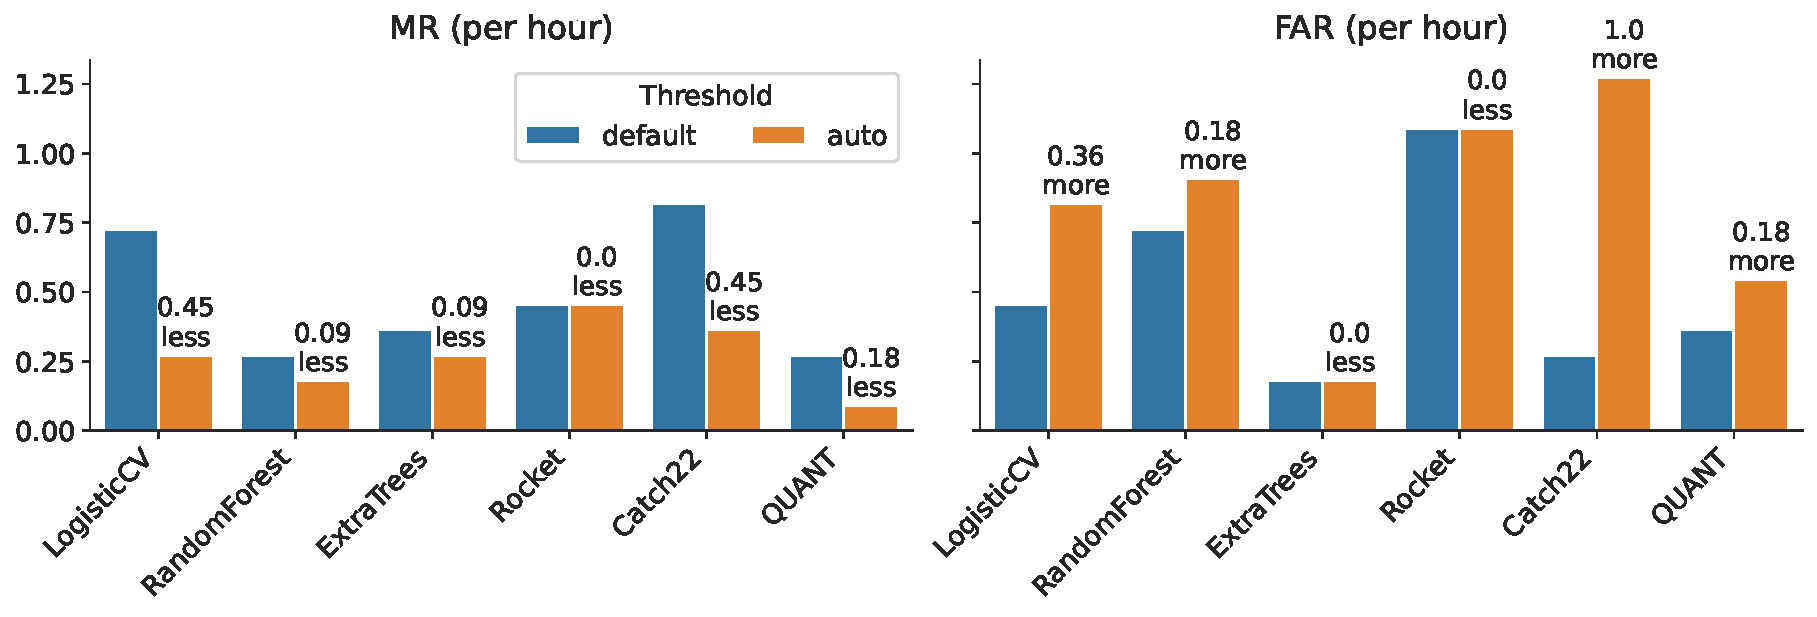
\includegraphics[width=\textwidth]{img/barplot_tune_threshold.pdf}
\caption{Effects of threshold tuning on false alarm rates and miss rates.} \label{fig:tune-thresh}
\end{figure}


\begin{table}[h]
\centering
\caption{Effects of cost-sensitive threshold tuning on FARSEEING.} \label{tab:tuning-results}
% \begin{tabular}{l c c c c c c c c}
\begin{tabularx}{0.9\textwidth}{l  @{\extracolsep{\fill}}  c  @{\extracolsep{\fill}}  c  @{\extracolsep{\fill}}  c  @{\extracolsep{\fill}}  c  @{\extracolsep{\fill}}  c @{\extracolsep{\fill}}  c @{\extracolsep{\fill}}  c @{\extracolsep{\fill}}  c}
\toprule
Model & $\tau$ & AUC & Precision & Recall & Specificity & F$_1$ & FAR & MR \\
\midrule
\multirow{2}{*}{Catch22} & 0.5 & 0.86 & 0.89 & 0.73 & 1.00 & 0.80 & 0.27 & 0.82 \\
 & auto & 0.94 & 0.67 & 0.88 & 1.00 & 0.76 & 1.27 & 0.36 \\
 \hline
\multirow{2}{*}{ExtraTrees} & 0.5 & 0.94 & \textbf{0.94} & 0.88 & 1.00 & 0.91 & \textbf{0.18} & 0.36 \\
 & auto & 0.95 & \textbf{0.94} & 0.91 & 1.00 & \textbf{0.92} & \textbf{0.18} & 0.27 \\ \hline
\multirow{2}{*}{LogisticCV} & 0.5 & 0.88 & 0.83 & 0.76 & 1.00 & 0.79 & 0.45 & 0.73 \\
 & auto & 0.95 & 0.77 & 0.91 & 1.00 & 0.83 & 0.82 & 0.27 \\ \hline
\multirow{2}{*}{QUANT} & 0.5 & 0.95 & 0.88 & 0.91 & 1.00 & 0.89 & 0.36 & 0.27 \\
 & auto & \textbf{0.98} & 0.84 & \textbf{0.97} & 1.00 & 0.90 & 0.55 & \textbf{0.09} \\ \hline
\multirow{2}{*}{RandomForest} & 0.5 & 0.95 & 0.79 & 0.91 & 1.00 & 0.85 & 0.73 & 0.27 \\
 & auto & 0.97 & 0.76 & 0.94 & 1.00 & 0.84 & 0.91 & 0.18 \\ \hline
\multirow{2}{*}{Rocket} & 0.5 & 0.92 & 0.70 & 0.85 & 1.00 & 0.77 & 1.09 & 0.45 \\
 & auto & 0.92 & 0.70 & 0.85 & 1.00 & 0.77 & 1.09 & 0.45 \\
\bottomrule
\end{tabularx}\\
Best results for each metric are shown in \textbf{bold}.
\end{table}

As shown in Table~\ref{tab:tuning-results}, threshold tuning generally improves F$_1$ scores and significantly reduces miss rates for most models without too much increase in false alarm rate. However, threshold tuning significantly increases false alarm rate for Catch22, and has no apparent effect on Rocket. 

\subsubsection{Further Validation.}
In this section, we further validate our technique by testing on MobiliseD, another real-world mobility dataset. We use a subset of Mobilised, which contains one subject with three reported real-world falls validated by domain experts. Following the structure of the FARSEEING dataset, we select a 20-minute signal around the annotated falls. For training, we use the full FARSEEING dataset, with the negative signals augmented with non-fall signals from Mobilised in order to appropriately tune the classifier thresholds. Then, we test the trained models on the three 20-minute signals obtained from MobiliseD.

\section{Discussion}

\section{Conclusion}

Of course, authors have complete freedom on how they choose to structure their paper. Section headers from Introduction up to and including Conclusions are completely up to the discretion of the authors; use whichever structure you see fit. Title, Abstract, the credits environment, and References, however, are mandatory.

\begin{credits}
\subsubsection{\ackname} A bold run-in heading in small font size at the end of the paper is
used for general acknowledgments, for example: This study was funded
by X (grant number Y).

\subsubsection{\discintname}
It is now necessary to declare any competing interests or to specifically
state that the authors have no competing interests. Please place the
statement with a bold run-in heading in small font size beneath the
(optional) acknowledgments,
for example: The authors have no competing interests to declare that are
relevant to the content of this article. Or: Author A has received research
grants from Company W. Author B has received a speaker honorarium from
Company X and owns stock in Company Y. Author C is a member of committee Z.
\end{credits}
%
% ---- Bibliography ----
%
% BibTeX users should specify bibliography style 'splncs04'.
% References will then be sorted and formatted in the correct style.
%
\bibliographystyle{splncs04}
\bibliography{refs}
%% Note that this preceding line implies that you store your BibTeX references in a file called 'mybibliography.bib'. If you instead store your references in a file with a different name, for instance 'references.bib', the preceding line should read '\bibliography{references}'. Whatever you do, DO NOT put the file name extension .bib inside the \bibliography command; this will trip up LaTeX compilers. 
%
% If you do not want to use BibTeX, you can also type up the bibliography exactly as you see fit, using the following structure:
% \begin{thebibliography}{8}
% % Note that this number 8 reserves an amount of space (equal to the natural width of the given number) for the label of your references; if you have more than 9 references, you will want to change this number to 18. If you have more than 19 references, this number is best changed to 88. If you have more than 99 references, I salute you.
% \bibitem{ref_article1}
% Author, F.: Article title. Journal \textbf{2}(5), 99--110 (2016)

% \bibitem{ref_lncs1}
% Author, F., Author, S.: Title of a proceedings paper. In: Editor,
% F., Editor, S. (eds.) CONFERENCE 2016, LNCS, vol. 9999, pp. 1--13.
% Springer, Heidelberg (2016). \doi{10.10007/1234567890}

% \bibitem{ref_book1}
% Author, F., Author, S., Author, T.: Book title. 2nd edn. Publisher,
% Location (1999)

% \bibitem{ref_proc1}
% Author, A.-B.: Contribution title. In: 9th International Proceedings
% on Proceedings, pp. 1--2. Publisher, Location (2010)

% \bibitem{ref_url1}
% LNCS Homepage, \url{http://www.springer.com/lncs}, last accessed 2023/10/25
% \end{thebibliography}
\end{document}
